\begin{figure*}[tp]
\centering
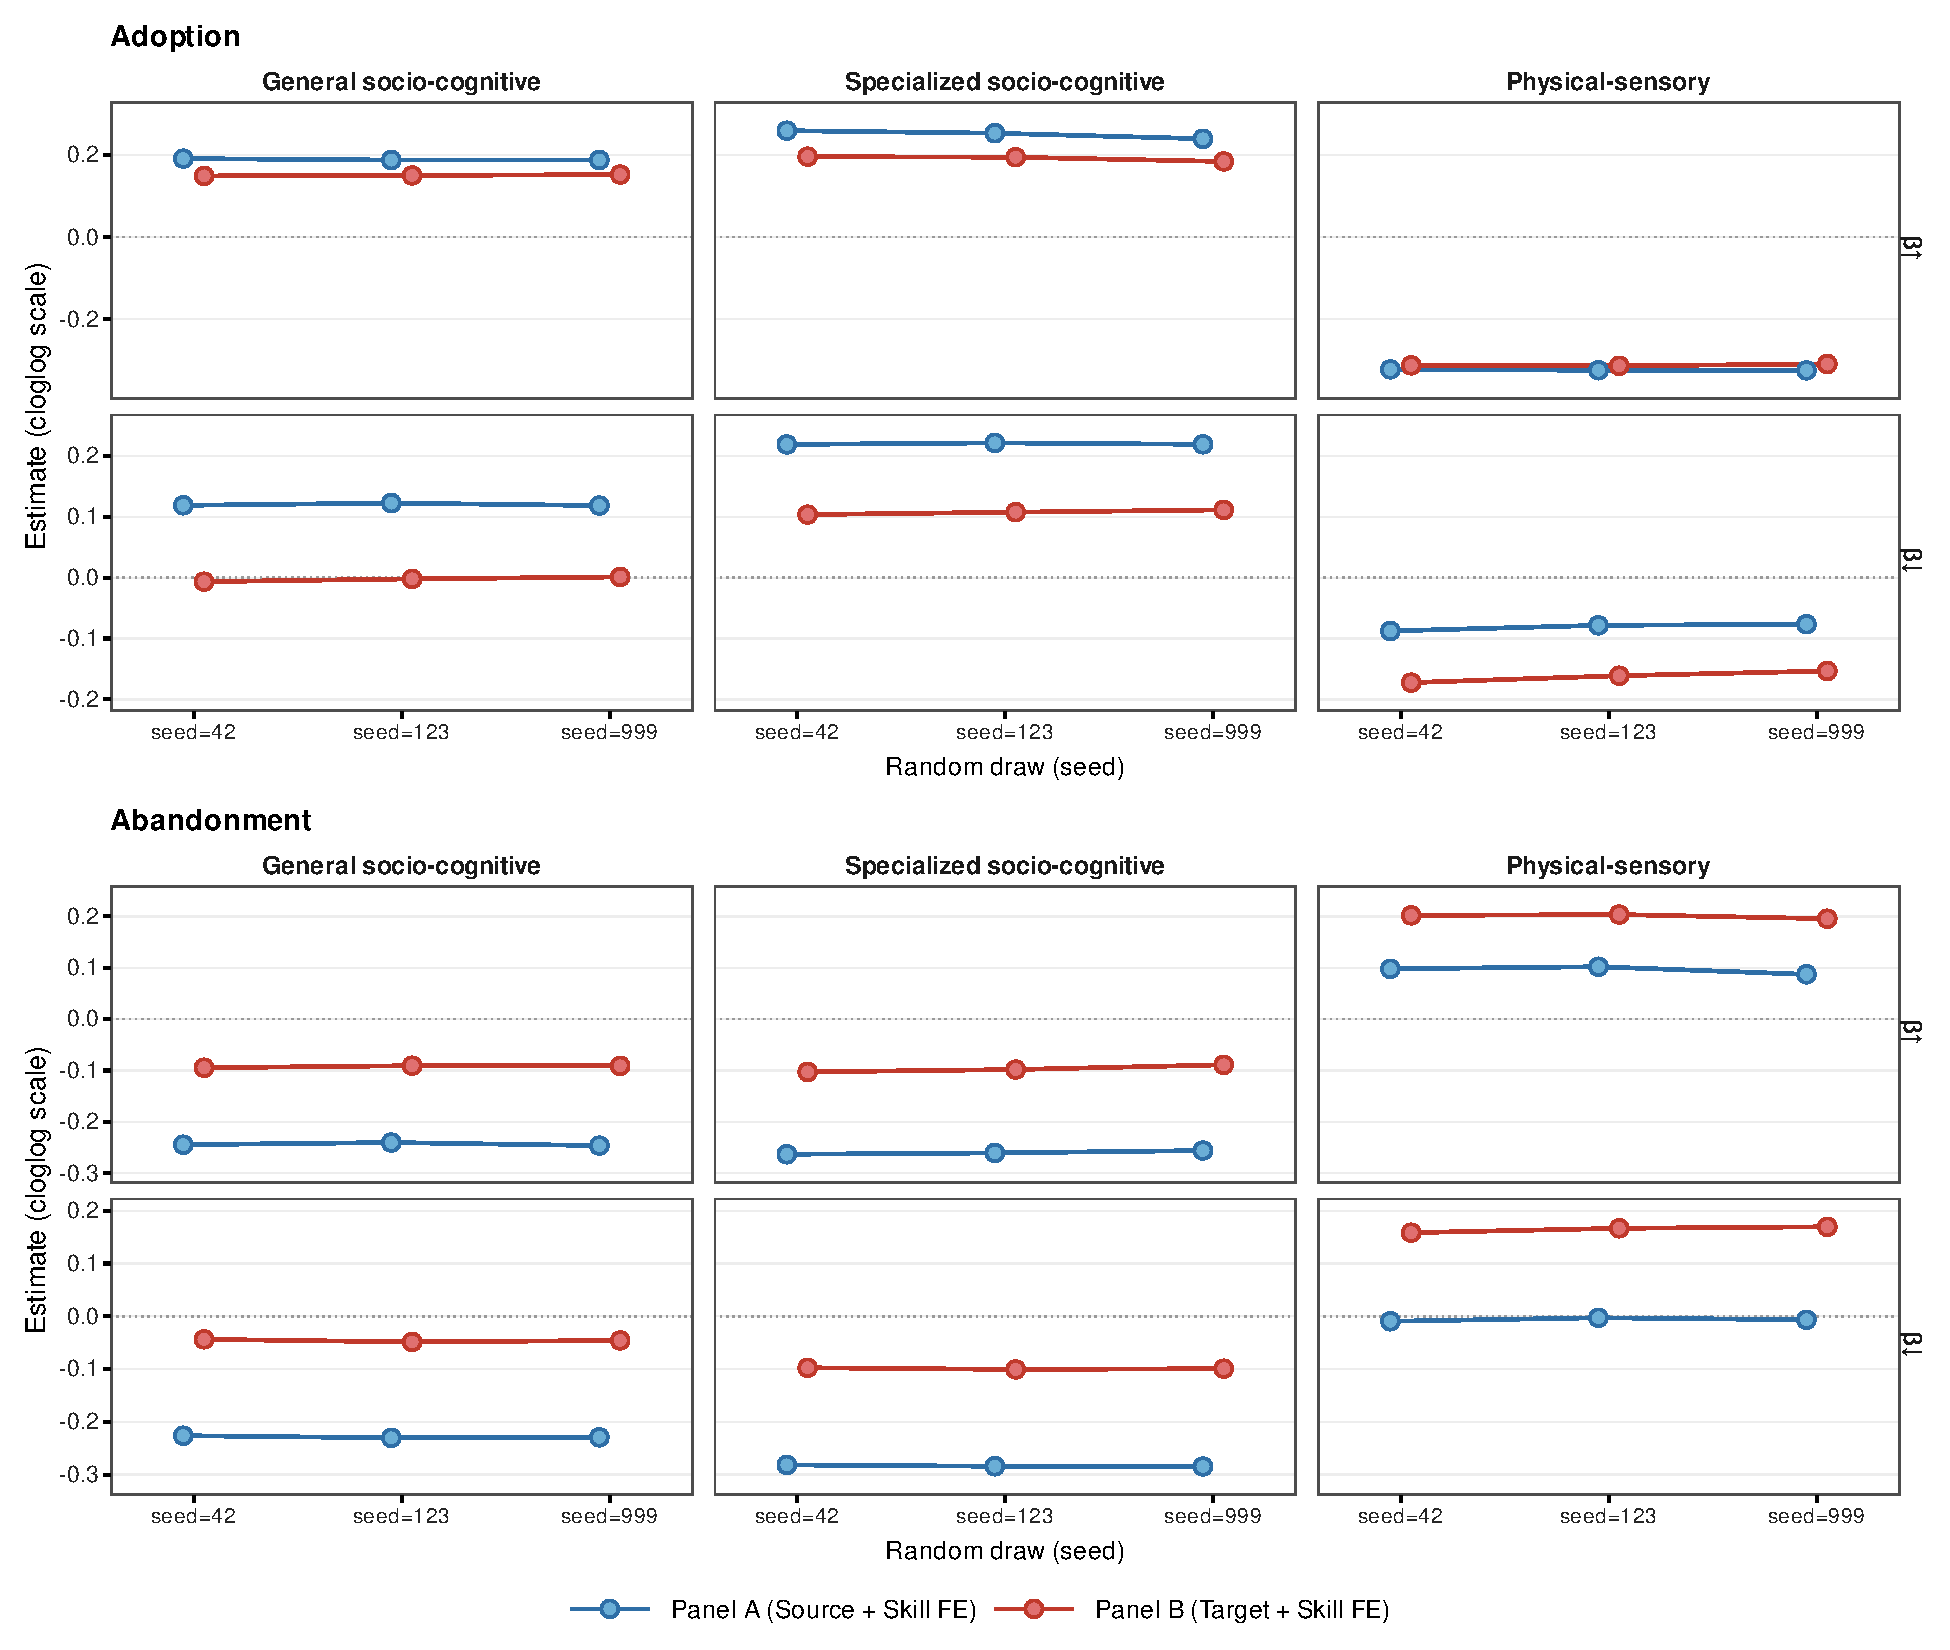
\includegraphics[width=0.95\textwidth]{figures/fig_SI_subsample_stability.pdf}
\caption{\textbf{Directional gravity estimates are stable across independent subsamples.} Each panel plots coefficient estimates from three independent 50\% random draws of source occupations (seeds 42, 123, 999). Rows correspond to $\hat{\beta}^{\uparrow}$ (top) and $\hat{\beta}^{\downarrow}$ (bottom); columns to skill type. Colors distinguish fixed-effect strategies. Near-flat lines indicate that estimates do not depend on the specific subsample drawn. The coefficient of variation across seeds is below 5\% in all cases. O*NET 2015--2024. \textbf{(A)} Adoption. \textbf{(B)} Abandonment.}
\label{fig:SI_stab}
\end{figure*}
